\chapter{树上问题初步}

树是最简单的图。序列可以视为一种特殊的树——链。相比序列，树失去了全序性质，分治结构也变得更加复杂。因此，树上问题往往要比序列问题复杂得多。

本章的依赖关系大致如下：先用有根树、祖先关系和 LCA 描述树上的结构；再用 DFS 序、欧拉序和链剖分把树上范围转化成序列上的范围；最后讨论直径、重心、差分等可以作为分治信息或维护信息的量。因此，前面出现 $\mathrm{lca}(u,v)$ 时只需要知道它表示 $u,v$ 的最近公共祖先，具体计算方法会在后文给出。

\section{树的基本性质}

无根树是一个无向图，具有以下几个基本性质：
\begin{itemize}
    \item 无环，连通
    \item 点数减边数等于 $1$
    \item 任意两点之间有且仅有一条路径
\end{itemize}

如果去除连通性要求，那么就得到森林。森林具有以下几个基本性质：
\begin{itemize}
    \item 无向无环图
    \item 连通块数等于点数减边数
    \item 任意两点之间至多有一条路径
\end{itemize}
    
第二条性质常常用来计算森林的连通块数，或者判断某个子图是否是树。
\begin{example}[ABC390F]
    给一个序列 $a$，定义区间 $[l,r]$ 的权值为 $a[l,r]$ 这些值形成的值域连续段个数。求所有区间的权值和。
\end{example}
\begin{exercise}
    给一棵树和一个序列 $a$，定义区间 $[l,r]$ 的权值为 $a[l,r]$ 在树上形成的导出子图连通块个数，求所有区间的权值和。
    \begin{hint}
        可以 $O(\min(u\text{ 的出现次数}, v\text{ 的出现次数})\log n)$ 计算一条边的贡献。
    \end{hint}
\end{exercise}
\begin{exercise}
    给一棵树和一个序列 $a$，定义区间 $[l,r]$ 的权值为 $a[l,r]$ 在树上形成的导出子图连通块个数。多次询问某个区间的权值和。
\end{exercise}
\begin{exercise}[[SDCPC 2019] Connected Intervals]
    给一棵树和一个序列 $a$，定义区间 $[l,r]$ 的权值为 $a[l,r]$ 在树上形成的导出子图连通块个数。求有多少个区间的权值为 $1$。
\end{exercise}

如果指定某一个点作为根，则得到有根树。有根树导出了一个偏序关系：父节点大于子节点。在这个偏序关系中，两个点可比（即 $x<y$ 或者 $x>y$）当且仅当它们之间有祖先后代关系。任意点集的公共祖先集合都是一条从根出发的链，其中深度最大的点称为它们的最近公共祖先（Lowest Common Ancestor，LCA）。有根树的深度定义为从根到该点的路径长度（有时也定义为路径上的点权和）。

\subsection{树的子结构}

树的常见子结构有以下几种：子树、路径/链、邻域。它们都是特殊的连通子图。

\begin{definition}
    在有根树中，\textbf{子树}是某个结点及其所有后代导出的子图。无根树的子树则是一个有歧义的概念，既可以指一个连通块，也可以指不包含某个点的极大连通块。因此，我们不对无根树使用这个术语。

    \textbf{路径/链}指的是某两个点之间的唯一路径。在有根树中，链可以分为直上直下的链和非直上直下的链两类。前者的性质通常与序列相似。任何一条链都可以由不超过两条直上直下的链拼起来得到。

    点 $u$ 的 $k$-\textbf{邻域}定义为距离 $u$ 不超过 $k$ 的点集。
\end{definition}

给定点集 $S$，在树上包含它们的最小连通块是唯一的，这个连通块通常被称为\textbf{虚树}。


\section{树的序列化}

可以通过某种方式遍历树来得到一个序列。根据遍历方式的不同，得到的序列会有不同的性质。

\subsection{DFS 序}

DFS 序是最常用的遍历顺序，它的性质是子树内的点在 DFS 序中是一段连续的区间。因此，可以通过这种方式将子树问题转为区间问题。不过，子树问题通常要比区间问题更容易。结点在 DFS 序中的位置通常用时间戳 \texttt{dfn[u]} 表示。



\subsection{BFS 序}

树的 BFS 序是用得比较少的遍历顺序。它的性质是一个点的所有孩子在 BFS 序中连续。对 BFS 序的一种更灵活的理解方式是把树按深度分层。

\begin{example}[邻域修改查询]
    给一棵树，支持把一个点的 $k$-邻域内的点权加，查询一个点的 $k$-邻域内的点权和。$k=O(1)$。
\end{example}
% \begin{solution}
%     对每一层深度分别按 BFS 序建立数据结构。固定点 $u$，按 $\mathrm{lca}(u,x)$ 是 $u$ 的第 $i$ 个祖先来分类，$i=0,\ldots,k$。在固定的深度层中，一个点的子树对应一段连续区间；若 $i>0$，还需要减去通向 $u$ 的那个儿子子树。因为 $k=O(1)$，一次邻域可以拆成 $O(k^2)$ 个“某一深度层上的子树区间”。
% \end{solution}

\subsection{欧拉序}

欧拉序是树按照一个“欧拉回路”访问点得到的顺序。在有根树中，可以这样得到一个欧拉序：
\begin{lstlisting}[language=C++]
void dfs(int u) {
    euler.push_back(u);
    for (int v : son[u]) {
        dfs(v);
        euler.push_back(u);
    }
}
\end{lstlisting}

\begin{property}
    在欧拉序中，取 $u$ 和 $v$ 的任意一对出现位置，则这两个位置之间的区间会包含 $u,v$ 链上的所有点的至少一次出现，且不包含 $\mathrm{lca}(u,v)$ 子树之外的点。因此，这段区间中深度最小的点全都是 $\mathrm{lca}(u,v)$。
\end{property}



\subsection{括号序}

括号序是在 DFS 进入和离开结点 $u$ 时分别写下 $u^+$ 和 $u^-$ 得到的序列。设 $l=\mathrm{lca}(u,v)$。括号序的性质是：假设 $u$ 在 $v$ 前被访问到，则括号序列在 $u^+$（不含）和 $v^+$（含）之间的部分抵消掉成对的 $w^+$ 和 $w^-$ 后，剩下的是 $[u,l)$ 这条链上的 $w^-$ 和 $(l,v]$ 这条链上的 $w^+$。通过这种方式可以把一些链上问题变成序列上的问题。

\begin{example}[括号序树链莫队]
    给一棵带颜色的树，多次询问一条链上有多少种出现次数为奇数的颜色。
\end{example}
% \begin{solution}
%     用括号序把每条链询问转成一个序列区间，再对这些区间做普通莫队。维护某个点在当前区间中出现了几次：出现两次的点会被抵消，出现一次的点正好对应询问链上的点。于是只需要像序列莫队一样维护颜色出现次数的奇偶性。
% \end{solution}
\begin{remark}
    完全的树链莫队需要树分块。
\end{remark}

\section{LCA 的计算}

有根树上的各种计算往往都需要 LCA。这里给出 LCA 的若干计算方式。

\subsection{向上跳}

首先考虑一个暴力：将深度更大的那个点向上跳到与另一个点深度相同，然后在两个点相遇之前不断地一起往上跳。我们可以通过一些手段优化这个暴力：

\begin{itemize}
    \item 倍增：预处理 $f_{i,j}$ 表示点 $i$ 向上跳 $2^j$ 步跳到的点即可。预处理 $O(n\log n)$，单次询问 $O(\log n)$，空间 $O(n\log n)$。
    \item 链剖分：在两个点跳到同一条链之前，每次让链顶深度更大的点向上跳到链顶的父亲；跳到同一条链之后返回深度小的点。通常使用重链剖分，此时预处理 $O(n)$，单次询问 $O(\log n)$，且常数较小。
\end{itemize}
\begin{remark}
    这两种方法较难做到 $O(1)$ 询问。倍增法的空间可以通过斜二倍增优化到 $O(n)$。
\end{remark}


\subsection{RMQ}

利用树的序列化可以将 LCA 问题变成 RMQ 问题。

\begin{itemize}
    \item 欧拉序：直接使用欧拉序找到两点在欧拉序中第一次出现的区间，然后在这个区间内查询深度最小的点。
    \item DFS 序：首先判断两点之间是否存在祖先后代关系；如果没有，那么两点在 DFS 序中对应的区间中深度最小的点的父亲即为 $\mathrm{lca}(u,v)$。
\end{itemize}

使用这种方法容易做到 $O(1)$ 询问。



\section{树的子结构的性质}

\subsection{子树}

在已知 $S$ 的导出子图连通的情况下，可以进一步检查
$$
    \sum_{u\in S}\deg(u)=2|S|-1.
$$
是否满足来判断 $S$ 是否为一个非整棵树的子树。

删去一个点集 $S$ 后，剩余图仍然连通，当且仅当 $S$ 的每个连通分量都至多通过一条边与 $V\setminus S$ 相连。等价地，若保留下来的点集 $C=V\setminus S$ 非空，则 $C$ 有唯一一个深度最小的点 $r_C$，且 $C$ 中任意点到 $r_C$ 的路径都完全包含在 $C$ 中；这时 $S$ 可以看成 $V\setminus \mathrm{subtree}(r_C)$ 加上若干个从 $C$ 上剪掉的完整子树。


\begin{exercise}[P8990]
\end{exercise}

子树之间要么包含，要么不交。反过来，具有这种性质的集合族也可以构建为一棵树。

\subsection{路径/链}


\begin{exercise}[判断点是否在链上]
    给定点 $u,v,x$，判断 $x$ 是否在 $u$ 到 $v$ 的链上。
\end{exercise}
\begin{solution}
    方法一：检查 $d(u,x)+d(x,v)=d(u,v)$。

    方法二：将链分解为两条直上直下的链上分别判断。直上直下的链上的判定可以转为子树判定，这可以通过 DFS 序实现。
\end{solution}

\begin{property}
    两条链的交要么是空集，要么仍然是一条链。具体来说，可以这样计算 $(u_1,v_1)$ 和 $(u_2,v_2)$ 的交：考虑 $\mathrm{lca}(u_1,u_2),\mathrm{lca}(u_1,v_2),\mathrm{lca}(v_1,u_2),\mathrm{lca}(v_1,v_2)$ 这四个点中按重数取深度最大的两个点 $u,v$（可能相同），那么链交要么是 $(u,v)$，要么是空集，可以通过判断 $u$ 是否同时在 $(u_1,v_1)$ 和 $(u_2,v_2)$ 上来区分。
\end{property}

\subsection{虚树}

点集 $S$ 的虚树有一个紧凑的刻画方式。
\begin{property}
    固定点集 $S$。树上的一个点 $u$ 为关键点当且仅当 $u\in S$，或者 $u$ 有至少两个儿子的子树与 $S$ 有交。一个关键点的父关键点定义为其祖先中深度最大的关键点。则 $S$ 的虚树是所有关键点和其父关键点之间的链的边不交并。把每条这样的链压成一条边，就得到通常意义下的虚树。
\end{property}
% \begin{example}[虚树的闭包]
    % 若 $1$ 的儿子为 $2,3$，$2$ 的儿子为 $4,5$，并取 $S=\{3,4,5\}$，则关键点集合为 $\{1,2,3,4,5\}$。虚树边为 $(1,2),(1,3),(2,4),(2,5)$，其中 $(1,2)$ 代表原树上的一整条链。
% \end{example}
\begin{exercise}
    令 $\bar S = \{\mathrm{lca}(u,v):u,v\in S\}$，说明关键点集合即为 $\bar S$。
\end{exercise}
\begin{exercise}
    证明关键点集合的大小不超过 $2|S|-1$。
\end{exercise}

\begin{example}[树上 TSP]
    给一棵树和一个点集 $S$，选择 $S$ 的一个排列 $u_1,\ldots,u_m$，分别使得
    \begin{itemize}
        \item $d(u_1,u_m)+\sum_{i=2}^m d(u_{i-1},u_i)$ 最小        
        \item $\sum_{i=2}^m d(u_{i-1},u_i)$ 最小
    \end{itemize}
\end{example}

\begin{example}[链并]
    给一棵树和树上的 $m$ 条链，将这些链的并集表示为 $O(m)$ 条不交的直上直下的链的并。
\end{example}

\section{树上差分与前缀和}

对于可差分的问题，可以将链用两类性质较好的集合表示：从根出发的链，以及子树。这两者互为对偶。

一条链可以表示为两条直上直下的链的不交并（且上端点大致相同），而直上直下的链又可以表示成两条从根出发的链的差。通过这种方式，我们可以把任意一条链表示为至多四条从根出发的链的加减。
% 例如，若 $F(u)=\sum_{x\in l_u} a_x$ 且 $p=\mathrm{lca}(u,v)$，则路径点权和为
% $$
%     \sum_{x\in P_{uv}}a_x=F(u)+F(v)-F(p)-F(\mathrm{fa}_p).
% $$
% 若维护的是边权，则变成写成 $F(u)+F(v)-2F(p)$。
% \begin{remark}
%     上式中约定 $F(\mathrm{fa}_{\mathrm{root}})=0$。
% \end{remark}

记 $l_v$ 为从根到 $v$ 的链，$s_u$ 为 $u$ 的子树，则 $u\in l_v$ 当且仅当 $v\in s_u$。通过这种方式，可以在这两种范围之间做对偶。例如，链加、查询单点可以对偶到单点加、查询子树和。

在 $\{l_u\}$ 结构上存在自然的前缀和与差分算子：$Sf(u)=Sf(\mathrm{fa}_u)+f(u)$，$Df(u)=f(u)-f(\mathrm{fa}(u))$，容易验证它们互逆。在 $\{s_u\}$ 结构上的前缀和与差分算子则更加复杂一些：$Sf(u)=f(u)+\sum_{v\in \mathrm{son}_u} Sf(v)$，$Df(u)=f(u)-\sum_{v\in \mathrm{son}_u} f(v)$。我们在组合数学课程中学习的前缀和与差分技巧也可以在这里使用。

\begin{exercise}[应用一]
    给定一个 LCA 黑盒。在 $O(1)$ 时间内查询一条链的点权和以及边权和，或者某个子树的点权和以及边权和。
\end{exercise}
\begin{exercise}
    据此得到一个 $O(1)$ 查询两点间距离的算法。
\end{exercise}

\begin{example}[应用二]
    给定一个 LCA 黑盒。在 $O(n+q)$ 时间内支持：一条链上的点权/边权加，某个子树内的点权/边权加，在所有修改结束后输出所有点权和边权。
\end{example}

\begin{example}[P4211]
    给一棵树，多次询问
    $$
    \sum_{i=l}^r f(\mathrm{lca}(i,x)).
    $$
    （假设有一个支持链修改查询的黑盒）
\end{example}
% \begin{solution}
%     令 $g(u)=f(u)-f(\mathrm{fa}_u)$，并约定 $f(\mathrm{fa}_{\mathrm{root}})=0$，则
%     $$
%         f(\mathrm{lca}(i,x))
%         =\sum_{y\in l_x,\ i\in s_y} g(y).
%     $$
%     按编号前缀离线处理。扫到点 $i$ 时，把根到 $i$ 的链上每个点的计数加一；询问前缀 $[1,r]$ 对 $x$ 的贡献时，在根到 $x$ 的链上查询 $\sum g(y)\cdot \mathrm{cnt}(y)$。区间 $[l,r]$ 的答案由两个前缀相减得到。
% \end{solution}
\begin{remark}
    此题还有线段树套虚树、点分树等做法。
\end{remark}



\section{直径}

树的直径定义为距离最远的两点之间的距离。这里距离定义为两个点之间唯一路径上的边权和/点权和/边权和与点权和的和。我们也把这样的两个点之间的路径称为直径。直径可能存在多条。
\begin{remark}
    在有负权时，这样定义的距离的性质通常比较差。如无特殊说明，我们默认树无负权。
\end{remark}
\begin{remark}
    在树退化成一条链的情况下，求直径相当于求最大子段和。这可以说明一些树上问题的困难性，如链加、查询直径。
\end{remark}

在确定直径后，可以将树画成以下的形式来帮助直观思考：

\begin{center}
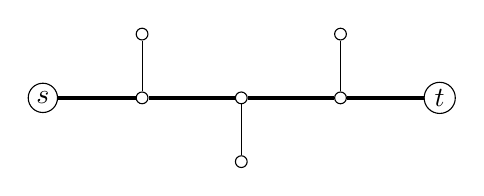
\begin{tikzpicture}[scale=0.9, every node/.style={circle, draw, inner sep=1.5pt}]
    \node (s) at (0,0) {$s$};
    \node (a) at (1.4,0) {};
    \node (b) at (2.8,0) {};
    \node (c) at (4.2,0) {};
    \node (t) at (5.6,0) {$t$};
    \node (x1) at (1.4,0.9) {};
    \node (x2) at (2.8,-0.9) {};
    \node (x3) at (4.2,0.9) {};
    \draw[very thick] (s)--(a)--(b)--(c)--(t);
    \draw (a)--(x1);
    \draw (b)--(x2);
    \draw (c)--(x3);
\end{tikzpicture}
\end{center}

有以下性质成立：

\begin{property}
    假设树无负权。任取一条直径 $(s,t)$，则对于任何一个点 $u$，$s,t$ 中至少有一个是距离 $u$ 最远的点之一。换句话说，距离一个点最远的点一定可以是直径的一个端点。
\end{property}
\begin{exercise}
    \begin{itemize}
        \item 说明在有负权时不成立。
        % 例如四点链 $a-b-c-d$ 的所有边权均为 $-1$，$(a,b)$ 是一条直径，但从 $d$ 出发的最远点是 $c$。
        \item 在边权和点权均非负，且距离 $d(u,v)$ 定义为路径上边权和加上 $u,v$ 两点的点权和时，证明该性质仍然成立。
    \end{itemize}
\end{exercise}
\begin{exercise}
    据此得到无负权树的直径的算法。
\end{exercise}
\begin{exercise}
    在有负权时，使用 DP 来计算直径。
\end{exercise}

下面的性质给出了连接两棵树后直径的变化。
\begin{property}
    假设树 $T_1$ 的一条直径是 $(s_1,t_1)$，树 $T_2$ 的一条直径是 $(s_2,t_2)$，并且边无负权。如果在两棵树中间加一条边得到一棵新树，那么新树中存在一条两个端点都在集合 $\{s_1,t_1,s_2,t_2\}$ 内的直径。
\end{property}
\begin{exercise}
    说明如何加边才能使得新树的直径最大/最小。
\end{exercise}
% \begin{solution}
%     若把 $x\in T_1$ 与 $y\in T_2$ 相连，则新直径长度为
%     $$
%         \max(D_1,D_2,\mathrm{ecc}_{T_1}(x)+c+\mathrm{ecc}_{T_2}(y)).
%     $$
%     因此最大化时连接两棵树各自的一个直径端点即可；最小化时连接两棵树的中心即可，此时答案为 $\max(D_1,D_2,R_1+c+R_2)$，其中 $R_i$ 是 $T_i$ 的半径。若题目只允许在原有顶点之间加边，则这里的中心和半径都取顶点意义下的最优值。
% \end{solution}
\begin{exercise}
    支持加边（保证任意时刻是森林）、查询某个连通块的直径。
\end{exercise}
% \begin{solution}
%     对每个连通块维护一组直径端点。合并两个连通块时，只需要在旧的四个端点之间枚举六对候选端点，取距离最大的一对作为新直径。
% \end{solution}
\begin{exercise}[P3596]
    给一棵树，对每条边，计算删除这条边然后再加一条新边后形成的树的直径可能的最大值和最小值。
\end{exercise}

对于边权为正的树，还有以下结论：
\begin{property}
    所有直径的中点（允许在边上）都相同。这个点称为树的中心（center），它最小化到树上所有点的最大距离。
\end{property}
\begin{remark}
    对于有零边的情况，可以把零边缩起来。
\end{remark}

\begin{exercise}[P1099/P2491]
    给定一棵非负权的树 $T$ 和一个常数 $s$，求一对点 $(u,v)$ 使得 $d(u,v)\le s$ 且 $\max_{x}\min_{y\in P_{uv}}d(x,y)$ 最小。也就是找到一条长度不超过 $s$ 的路径，使得到这条路径的最远距离最小。需要 $O(n)$。
\end{exercise}
\begin{exercise}[P3304]
    询问有多少条边满足所有的直径都经过它。
\end{exercise}

我们也可以定义一个点集内的直径。对于点集 $S$，定义 $S$ 内的直径为 $S$ 中距离最远的两点之间的距离。此时，有以下性质成立。
\begin{property}
    假设树无负权。任取点集 $S$ 内的一条直径 $(s,t)$，则对于树上的任何一个点 $u$，$s,t$ 中至少有一个是 $S$ 内距离 $u$ 最远的点之一。 
\end{property}
\begin{exercise}
    证明以下结论：任取点集 $S_1$ 内的一条直径 $(s_1,t_1)$ 和点集 $S_2$ 内的一条直径 $(s_2,t_2)$，则 $S_1\cup S_2$ 内存在一条两个端点都在 $\{s_1,t_1,s_2,t_2\}$ 内的直径。因此，点集内的直径是一种可以快速合并的分治信息。
\end{exercise}
\begin{exercise}
    多次询问 $S=[l,r]$ 内的直径。
\end{exercise}
\begin{exercise}
    给一棵树，维护一个点集 $S$，支持添加/删除点到 $S$ 中，查询 $S$ 内的直径。
\end{exercise}
\begin{remark}
    有负权时可以通过动态 DP 之类的方法做到 $O(\log n)$，参见 P4115。
\end{remark}
\begin{example}[CF1192B]
    修改边权，查询直径。保证边权非负。
\end{example}
\begin{remark}
    如果没有边权非负的保证，那么可以用静态 Top Tree 等方法做到 $O(\log n)$。
\end{remark}

\section{重心}

假设树 $T$ 带有非负的点权，且总点权大于零。定义一个点集 $S$ 的重量 $w(S)$ 为该点集内的点权和。树的重心（median/centroid）有以下两个等价定义：
\begin{itemize}
    \item 以重心 $u$ 为根时，$\max_{v\in \mathrm{son}_u}w(\mathrm{subtree}(v))$（最大的子树重量）最小。
    \item 以重心 $u$ 为根时，任何 $v\ne u$ 都满足 $w(\mathrm{subtree}(v)) \le w(T)/2$（每个子树的重量都不超过总重量的一半）。
\end{itemize}
\begin{remark}
    注意重心未必在直径上。
\end{remark}
直观上，重心可以这样取得：假设当前在点 $u$，考虑删掉 $u$ 形成的所有连通块，如果存在重量 $>w(T)/2$ 的那么就往这个连通块移动，否则 $u$ 本身就是重心。利用这个直观，我们可以得到以下性质：
\begin{property}
    \begin{itemize}
        \item 对一棵以 $r$ 为根的树，若 $r$ 不是重心，则存在唯一一个重量 $>w(T)/2$ 的儿子子树，并且所有重心都在这棵子树中。
        \item 假设 $u$ 是树的重心，并把树以 $u$ 为根。那么树除了 $u$ 之外的所有重心，恰好是满足 $w(\mathrm{subtree}(v))=w(T)/2$ 的点 $v$。在点权均为正的情况下，这样的点 $v$ 至多只有一个，故此时重心至多有两个且二者相邻。
    \end{itemize}
\end{property}

对于一棵以 $r$ 为根的有根树，在切换到以 $u$ 为根时，除了原本的子树外，还会产生一个“向上”的子树，这个子树的重量为 $w(T)-w(\mathrm{subtree}(u))$。可以据此判定一个点是否为树的重心。
\begin{exercise}[P5666]
    给一棵树，计算删除每条边后，形成的两个连通块中的所有重心的编号之和。
\end{exercise}

下面的性质将重心与距离联系在一起。
\begin{property}
    假设树的边权非负，距离定义为两点之间的路径的边权和。树的重心可以最小化所有点到它的距离之和，即 $\sum_v w_v \cdot d(v, u)$。
\end{property}
也可以据此定义点集内的重心：
\begin{definition}
    对于点集 $S$，定义 $S$ 内的重心为距离 $S$ 内所有点的距离之和最小的 $S$ 内的点，即 $\arg\min_{u \in S} \sum_{v \in S} w_v \cdot d(u, v)$。这里距离定义为两点之间路径上的边数（事实上任何非负边权导出的距离都可行）。
\end{definition}



下面的性质说明了连接两棵树后重心的变化情况。
\begin{property}
    假设树 $T_1,T_2$ 的点权均为正，且 $u_1,u_2$ 分别是它们的一个重心。如果在两棵树中间加一条边得到一棵新树，那么新树的所有重心都在 $u_1$ 和 $u_2$ 之间的链上。
\end{property}
\begin{example}[P4299]
    加边（保证任意时刻是森林），查询连通块重心。
\end{example}

下面的性质给出了重心与 DFS 序的联系。
\begin{property}
    DFS 序的带权中点定义为满足 $\sum_{i<k} w_{p_i} \le \frac{W}{2}$ 且 $\sum_{i>k}^n w_{p_i} \le \frac{W}{2}$ 的 $k$。这样的 $p_k$ 在深度最小的那个重心的子树内。
\end{property}
\begin{exercise}
    子树点权加/赋值，查询重心。
\end{exercise}
\begin{remark}
    后面我们学习链剖分之后还能支持链修改。
\end{remark}
\begin{exercise}
    查询 $S=[l,r]$ 内的重心。
\end{exercise}
\begin{solution}
    通过可持久化线段树/整体二分之类的方法求出 $S$ 在 DFS 序中的带权中点，然后从那个点向上跳到最后一个子树内有至多 $w(S)/2$ 重量的点即可。
\end{solution}

\section{链剖分}

%TODO

链剖分把树分解为若干条直上直下的链。可以让每个结点选择至多一个孩子作为特殊孩子，对应的边为特殊边，则这些特殊边将树划分为若干直上直下的链。根据选择特殊边的方式不同，可以得到以下几种链剖分：

\begin{itemize}
    \item 重链剖分：每个结点选择子树大小最大的儿子作为特殊儿子。
    \item 长链剖分：每个结点选择子树深度最大（指从根到最深叶子的长度）的儿子作为特殊儿子。
    \item 任意链剖分：每个结点选择任意一个儿子作为特殊儿子。
\end{itemize}


，使得一条任意链可以被分解成少量连续片段。最常用的是重链剖分：对每个非叶结点，选择一个子树大小最大的儿子作为重儿子，连向重儿子的边称为重边，其它边称为轻边。重边连成的极大链称为重链。

\begin{property}
    在重链剖分中，任意根到点的路径上经过的轻边数为 $O(\log n)$。
\end{property}
\begin{proof}
    如果 $(u,v)$ 是轻边且 $v$ 是 $u$ 的儿子，那么还存在一个重儿子 $h$ 满足 $\mathrm{size}(h)\ge \mathrm{size}(v)$，所以 $\mathrm{size}(v)\le(\mathrm{size}(u)-1)/2$。每经过一条轻边，当前子树大小至少减半，因此轻边数为 $O(\log n)$。
\end{proof}

把每条重链按照从上到下的顺序接到 DFS 序中，就能保证一条重链对应一个连续区间。任意树链可以通过不断跳链顶分解成 $O(\log n)$ 个连续区间，从而交给线段树、树状数组或其它序列数据结构维护。

\begin{example}[树链修改查询]
    支持链加、链求和、子树加、子树求和。
\end{example}
\begin{solution}
    子树在 DFS 序中本来就是一个连续区间。链操作则用重链剖分拆成 $O(\log n)$ 个 DFS 序区间。于是只要底层序列数据结构支持区间加和区间求和即可。
\end{solution}
